\section{PART 1: APPLY ALGORITHMS TO TWO PROBLEMS}
\subsection{Experiment Setup}
This project was implemented using Python version 3.11.9 and the mlrose \cite{Hayes19} package to apply various search algorithms to the randomized optimization problems. All simulations were conducted on a system equipped with an AMD Ryzen 9 6900HS processor, 15.2 GB of usable RAM, and executed in an interactive notebook environment. For each algorithm, the default parameters provided by the mlrose library were used, with only one parameter being varied at a time to observe its influence on the algorithm's performance. During each run, the wall clock time, best fitness values, and the fitness curve were recorded to evaluate the performance of each algorithm. Multiple plots were generated to visualize the impact of the parameter changes on the optimization process and to compare the performance across different search runs.
\subsection{Traveling Salesman Problem (TSP)}
The TSP \cite{LAPORTE1992231} is a well-known NP-hard optimization problem where the objective is to find the shortest possible route that visits a set of cities exactly once and returns to the starting city. Due to the vast number of possible routes, especially as the number of cities increases, traditional optimization methods often struggle with local optima, making it difficult to find globally optimal solutions. This complexity makes the TSP an excellent problem for demonstrating the strengths of randomized optimization algorithms, particularly Simulated Annealing (SA), which is designed to escape local optima by allowing controlled random fluctuations in the solution space.

In this implementation, I used 50 cities, where each city is represented as a point with randomly generated distances between every pair of cities. The distances were generated using a random floating-point value between 0.0 and 1.0 for each pair of cities. The cities were positioned using randomly generated (x,y) coordinates within a specified range, and a set of nearby points was excluded from the random generation process to ensure diversity in city locations. To model the TSP problem, the mlrose library was used, and the TravellingSales fitness function was applied, which evaluates the total distance of a given route. The TSP was then formulated as an optimization problem using the TSPOpt class, where the goal was to minimize the total travel distance.

My hypothesis for this problem was that SA, due to its exploration abilities, should provide the best fitness score by finding near-optimal routes while avoiding local optima more effectively than other algorithms. For each run, I observed the best fitness score (representing the shortest total distance), the wall clock time for the optimization process, and the fitness curve (Figure~\ref{fig:tspgrid}) that tracks the progression of solutions across iterations. Each run was set for a maximum of 1000 iterations. For SA (Figure~\ref{fig:tspsa}), I tested exponential cooling of 0.001, 0.005, and 0.01, with the best fitness achieved using 0.001. For RHC (Figure~\ref{fig:tsprhc}), I tested restart values of 0, 5, and 10, and found that 0 and 5 yielded the best results. For the Genetic Algorithm (GA) (Figure~\ref{fig:tspga}), population sizes of 100, 200, and 300 were tested, with 100 providing the best fitness. For MIMIC (Figure~\ref{fig:tspmimic}), I tested population sizes of 100, 200, and 
300, and found that both 100 and 200 produced strong results.

From Figure~\ref{fig:tspbest}, we observe that MIMIC achieved the best fitness score of 16.9, closely followed by SA with 14.19. I previously hypothesized that SA would achieve the best fitness for this problem because of its strong exploration capabilities, which allow it to escape local optima. However, MIMIC outperformed SA. This could be because MIMIC employs a probabilistic model that captures dependencies between variables more effectively, leading to better exploration of the solution space. Additionally, MIMIC’s larger population sizes may have allowed it to find more global solutions, albeit at the cost of computational time. The Genetic Algorithm (GA) performed the worst, with a best fitness of 9.14, followed closely by RHC with 12.83.

In terms of efficiency, we can observe from Figure~\ref{fig:tspgrid} that SA reaches its best fitness score in around 1500 iterations, while MIMIC requires over 6000 iterations to reach its best score. This demonstrates SA's strength in quickly finding good solutions due to its ability to accept worse solutions early on, allowing it to explore a wide variety of routes before cooling down. The wall clock time for each algorithm is plotted in Figure~\ref{fig:tsptime}. We see that SA achieves its result in around 0.32 seconds, while MIMIC takes significantly longer, requiring 21.66 seconds to complete the run. This disparity in time highlights a critical trade-off: although MIMIC finds the best fitness, it is computationally expensive, making it less suitable for this problem. The trend of the fitness curve (Figure~\ref{fig:tspsa}  with SA shows that decreasing the exponential cooling even further, SA would achieve even higher fitness scores.

\begin{figure*}[htbp]
    \centering
    \begin{subfigure}[b]{0.49\textwidth}
        \centering
        \includegraphics[width=\textwidth]{image/part-1/tsp/rhc.png}
        \caption{}
        \label{fig:tsprhc}
    \end{subfigure}
    \hfill
    \begin{subfigure}[b]{0.49\textwidth}
        \centering
        \includegraphics[width=\textwidth]{image/part-1/tsp/sa.png}
        \caption{}
        \label{fig:tspsa}
    \end{subfigure}
    \vskip\baselineskip
    \begin{subfigure}[b]{0.49\textwidth}
        \centering
        \includegraphics[width=\textwidth]{image/part-1/tsp/ga.png}
        \caption{}
        \label{fig:tspga}
    \end{subfigure}
    \hfill
    \begin{subfigure}[b]{0.49\textwidth}
        \centering
        \includegraphics[width=\textwidth]{image/part-1/tsp/mimic.png}
        \caption{}
        \label{fig:tspmimic}
    \end{subfigure}
    \caption{Fitness vs. iterations for the TSP using different randomized optimization algorithms: (a) Randomized Hill Climbing, (b) Simulated Annealing, (c) Genetic Algorithm, and (d) MIMIC. The plots show the impact of varying key parameters—restarts for RHC, exponential cooling for SA, population sizes for GA, and population sizes for MIMIC—on the fitness progression over iterations.}
    \label{fig:tspgrid}
\end{figure*}
\begin{figure}[htbp]
\centerline{\includegraphics[width=1\linewidth]{image/part-1/tsp/best.png}}
\caption{Fitness vs. iterations for the best-performing parameters of different optimization algorithms on the TSP. The plot compares RHC, SA, GA, and MIMIC. The fitness progression over time highlights the effectiveness of each algorithm, with SA showing volatile behavior but strong performance early, and GA and MIMIC gradually converging to better solutions over longer iterations.}
\label{fig:tspbest}
\end{figure}
\begin{figure}[htbp]
    \centering
    \begin{subfigure}[b]{0.48\textwidth}
        \centering
        \includegraphics[width=\textwidth]{image/part-1/tsp/fitness bins.png}
        \caption{}
        \label{fig:tspfitbins}
    \end{subfigure}
    \vskip\baselineskip
    \begin{subfigure}[b]{0.48\textwidth}
        \centering
        \includegraphics[width=\textwidth]{image/part-1/tsp/time.png}
        \caption{}
        \label{fig:tsptime}
    \end{subfigure}
    \caption{Performance comparison of different optimization algorithms on the TSP in terms of (a) best fitness achieved and (b) wall clock time. The results demonstrate the trade-offs between solution quality and computational time for each algorithm.}
    \label{fig:tspfitbinstimegrid}
\end{figure}

\subsection{Four Peaks Problem (FPP)}
The FPP is a deceptive optimization problem that involves finding a bitstring that maximizes the length of consecutive 0's followed by consecutive 1's (or vice versa), with an additional bonus for reaching a certain threshold. This bonus is given if the number of consecutive leading 0's and trailing 1's both exceed a defined threshold t, which is based on a percentage of the total string length. This creates two regions of interest: one for maximizing the leading 0's and one for maximizing the trailing 1's. The deceptive nature of the problem lies in the fact that maximizing one sequence (either 0's or 1's) without considering the threshold can trap the optimization in suboptimal solutions, making the problem challenging for traditional search methods.

For this experiment, the bonus is set to 50 points, and to achieve this bonus, the binary string must have at least 8 leading 0's and 8 trailing 1's, as the threshold percentage 0.15 results in a threshold of 8. The maximum fitness score that can be attained is 100: 25 points for the leading 0's, 25 points for the trailing 1's, and a bonus of 50 when the threshold is satisfied.

My hypothesis is that the GA would perform best on this problem because GA tends to explore a wider range of solutions through crossover and mutation, making it more capable of escaping local optima compared to other algorithms. For each run, I observed the best fitness score (representing the most optimal bitstring found), the wall clock time for the optimization process, and the fitness curve (Figure~\ref{fig:fppgrid}) that tracks the progression of solutions across iterations.

Each run was set for a maximum of 1000 iterations. For SA (Figure~\ref{fig:fppsa}), I tested exponential cooling schedules with rates of 0.001, 0.005, and 0.01, with the best fitness achieved using a cooling rate of 0.001. For Randomized Hill Climbing (RHC) (Figure~\ref{fig:fpprhc}), I tested restart values of 0, 5, and 10, and found that restarts of 5 and 10 produced the best results. For the Genetic Algorithm (GA) (Figure~\ref{fig:fppga}), I experimented with population sizes of 100, 200, and 300, with 100 providing the best fitness. For MIMIC (Figure~\ref{fig:fppmimic}), I tested population sizes of 100, 200, and 300, and found that 300 produced strong results.

From Figure~\ref{fig:fppga}, we can observe that for all runs with varying population sizes, GA consistently achieves the best fitness score, consistently reaching above 70. No other algorithm comes close to this performance except for MIMIC (Figure~\ref{fig:fppmimic})), which achieves a similar score with a population size of 300. RHC in Figure~\ref{fig:fpprhc} consistently performs poorly across all variations of restart values. At a restart value of 0, RHC is unable to find a solution and gets stuck in an early local optimum. Increasing the restarts to 5 and 10 helps marginally, allowing the algorithm to escape the early local optima, but it still converges to a suboptimal solution with a fitness score of 6. SA (Figure~\ref{fig:fppsa}) performs better than RHC, reaching a best fitness of 37, but still falls short compared to GA and MIMIC. As previously stated, GA escapes early local optima and demonstrates strong performance with a best fitness of 72, achieving this score in under 1000 iterations. MIMIC performs poorly at lower population sizes of 100 and 200, but as the population size is increased to 300, it begins to approach the performance of GA, achieving a best fitness score of 72 (Figure~\ref{fig:fppbest}). This could be due to MIMIC's probabilistic model capturing more global information as the population size increases, enabling better exploration of the solution space.

In terms of efficiency, as measured by wall clock time (Figure~\ref{fig:fpptime}), we can deduce that the optimization times for RHC, SA, and GA are relatively low, ranging between 0.02 and 0.37 seconds. However, MIMIC takes significantly longer, requiring 26.52 seconds to complete its run. The increased time required by MIMIC is likely due to the complexity of its model-building process and the larger population sizes involved, which slow down convergence.
\begin{figure*}[htbp]
    \centering
    \begin{subfigure}[b]{0.49\textwidth}
        \centering
        \includegraphics[width=\textwidth]{image/part-1/four peaks/rhc.png}
        \caption{}
        \label{fig:fpprhc}
    \end{subfigure}
    \hfill
    \begin{subfigure}[b]{0.49\textwidth}
        \centering
        \includegraphics[width=\textwidth]{image/part-1/four peaks/sa.png}
        \caption{}
        \label{fig:fppsa}
    \end{subfigure}
    \vskip\baselineskip
    \begin{subfigure}[b]{0.49\textwidth}
        \centering
        \includegraphics[width=\textwidth]{image/part-1/four peaks/ga.png}
        \caption{}
        \label{fig:fppga}
    \end{subfigure}
    \hfill
    \begin{subfigure}[b]{0.49\textwidth}
        \centering
        \includegraphics[width=\textwidth]{image/part-1/four peaks/mimic.png}
        \caption{}
        \label{fig:fppmimic}
    \end{subfigure}
    \caption{Fitness vs. iterations for the FPP using different randomized optimization algorithms: (a) Randomized Hill Climbing, (b) Simulated Annealing, (c) Genetic Algorithm, and (d) MIMIC. The plots show the impact of varying key parameters—restarts for RHC, exponential cooling for SA, population sizes for GA, and population sizes for MIMIC—on the fitness progression over iterations.}
    \label{fig:fppgrid}
\end{figure*}
\begin{figure}[htbp]
\centerline{\includegraphics[width=1\linewidth]{image/part-1/four peaks/best.png}}
\caption{Fitness vs. iterations for the best-performing parameters of different optimization algorithms on the FPP. The plot compares RHC, SA, GA, and MIMIC. The fitness progression over time highlights the effectiveness of each algorithm, with SA showing volatile behavior but strong performance early, and GA and MIMIC gradually converging to better solutions over longer iterations.}
\label{fig:fppbest}
\end{figure}
\begin{figure}[htbp]
    \centering
    \begin{subfigure}[b]{0.48\textwidth}
        \centering
        \includegraphics[width=\textwidth]{image/part-1/four peaks/fitness bins.png}
        \caption{}
        \label{fig:fppfitbins}
    \end{subfigure}
    \vskip\baselineskip
    \begin{subfigure}[b]{0.48\textwidth}
        \centering
        \includegraphics[width=\textwidth]{image/part-1/four peaks/time.png}
        \caption{}
        \label{fig:fpptime}
    \end{subfigure}
    \caption{Performance comparison of different optimization algorithms on the FPP in terms of (a) best fitness achieved and (b) wall clock time. The results demonstrate the trade-offs between solution quality and computational time for each algorithm.}
    \label{fig:fppfitbinstimegrid}
\end{figure}